\chapter{Oracle APEX}

\section{Pengertian Oracle APEX}
Oracle Apex (Application Express) merupakan sebuah Aplikasi database berbasis web yang digunakan dalam database Oracle. Oracle Apex ini hanya menggunakan web browser saja dan proses pemrograman yang sederhana, serta mengembangkan ilmu dan kemampuan dengan Aplikasi ini aman dan cepat. Aplikasi Oracle Apex ini memiliki kualitas database yang bagus, produktifitas dan standart luas yang dimiliki oleh perusahaan – perusahaan besar dan memiliki keamanan, stabilitas, ketersediaan dalam membangun suatu web. Aplikasi ini merupakan suatu alat yang digunakan untuk membangun Aplikasi web- Based. Selain itu Oracle Apex tidak membutuhkan perangkat lainnya untuk mengembangkan, menyebarkan, serta menjalankan aplikasi, karena di dalam Oracle Apex ini telah menyediakan tiga alat utama seperti : 
\begin{enumerate}
    \item Application Builder : Yang digunakan untuk membuat aplikasi, melihat aplikasi, mengimport aplikasi, mengatur service, mengatur user aplikasi dan memantau aktifitas yang dilakukan pengguna.
    \item SQL Workshop : Yang digunakan untum membuat table dan komponennya (menggnakan kode PL – SQL secara manual maupun otomatis), melihat struktur table dan komponennya, mengimpor dan mengekspor script.
    \item Utilitas : Yang digunakan untuk melihat report table dan komponennya serta history aplikasi.
\end{enumerate}


\section{Tahapan Membuat Aplikasi Oracle Apex}
Pertama kita buka websitenya yaitu https://apex.oracle.com, kita akan mendapatkan akses untuk memasuki Oracle Apllication Express, masukan email anda yang valid untuk membuat Workspace,  bagaimana tahapan pembuatan Aplikasi pada Oracle APEX :
\begin{enumerate}
    \item Pergi ke halaman website https://apex.oracle.com/
           \begin{figure}[!htbp]
    \centering
    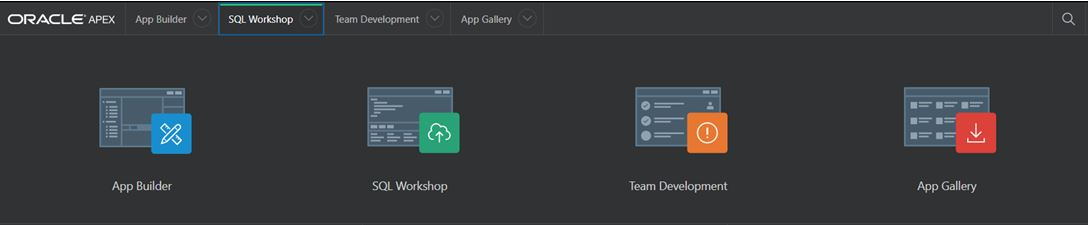
\includegraphics[scale=0.4]{section/2.JPG}
    \label{gambar 1}
\end{figure}

\item Sign in akun anda yang baru saja di buat lalu masuk ke App Builder setelah itu buat App Baru lalu klik create untuk membuat
       \begin{figure}[!htbp]
    \centering
    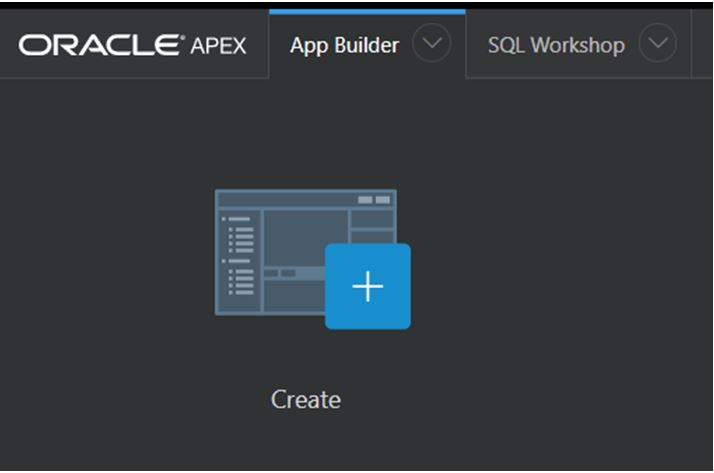
\includegraphics[scale=0.4]{section/3.JPG}
    \label{gambar 1}
\end{figure}

\item Lalu klik from a file dari sebuah file.
       \begin{figure}[!htbp]
    \centering
    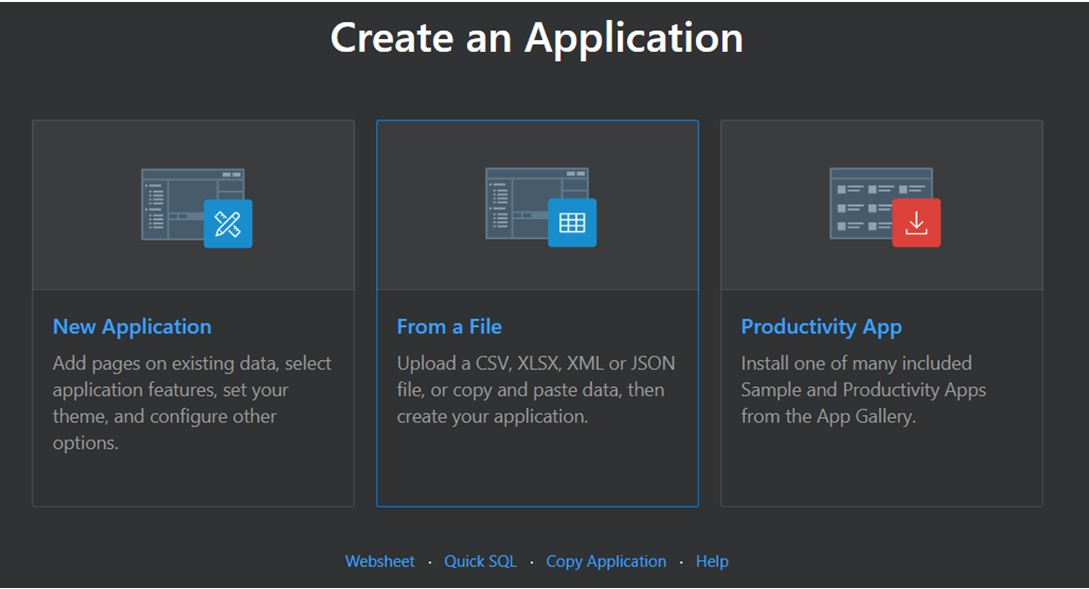
\includegraphics[scale=0.5]{section/4.JPG}
    \label{gambar 1}
\end{figure}
\item Klik Choose file
       \begin{figure}[!htbp]
    \centering
    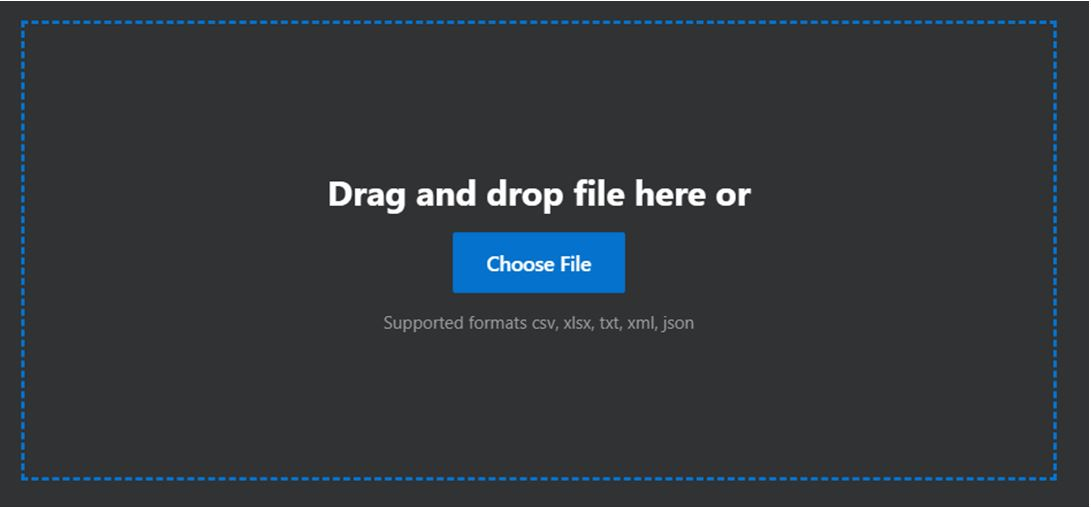
\includegraphics[scale=0.4]{section/5.JPG}
    \label{gambar 1}
\end{figure}
\vspace{3cm}
\item Masuk ke table name dan isi dengan akademik sederhana
       \begin{figure}[!htbp]
    \centering
    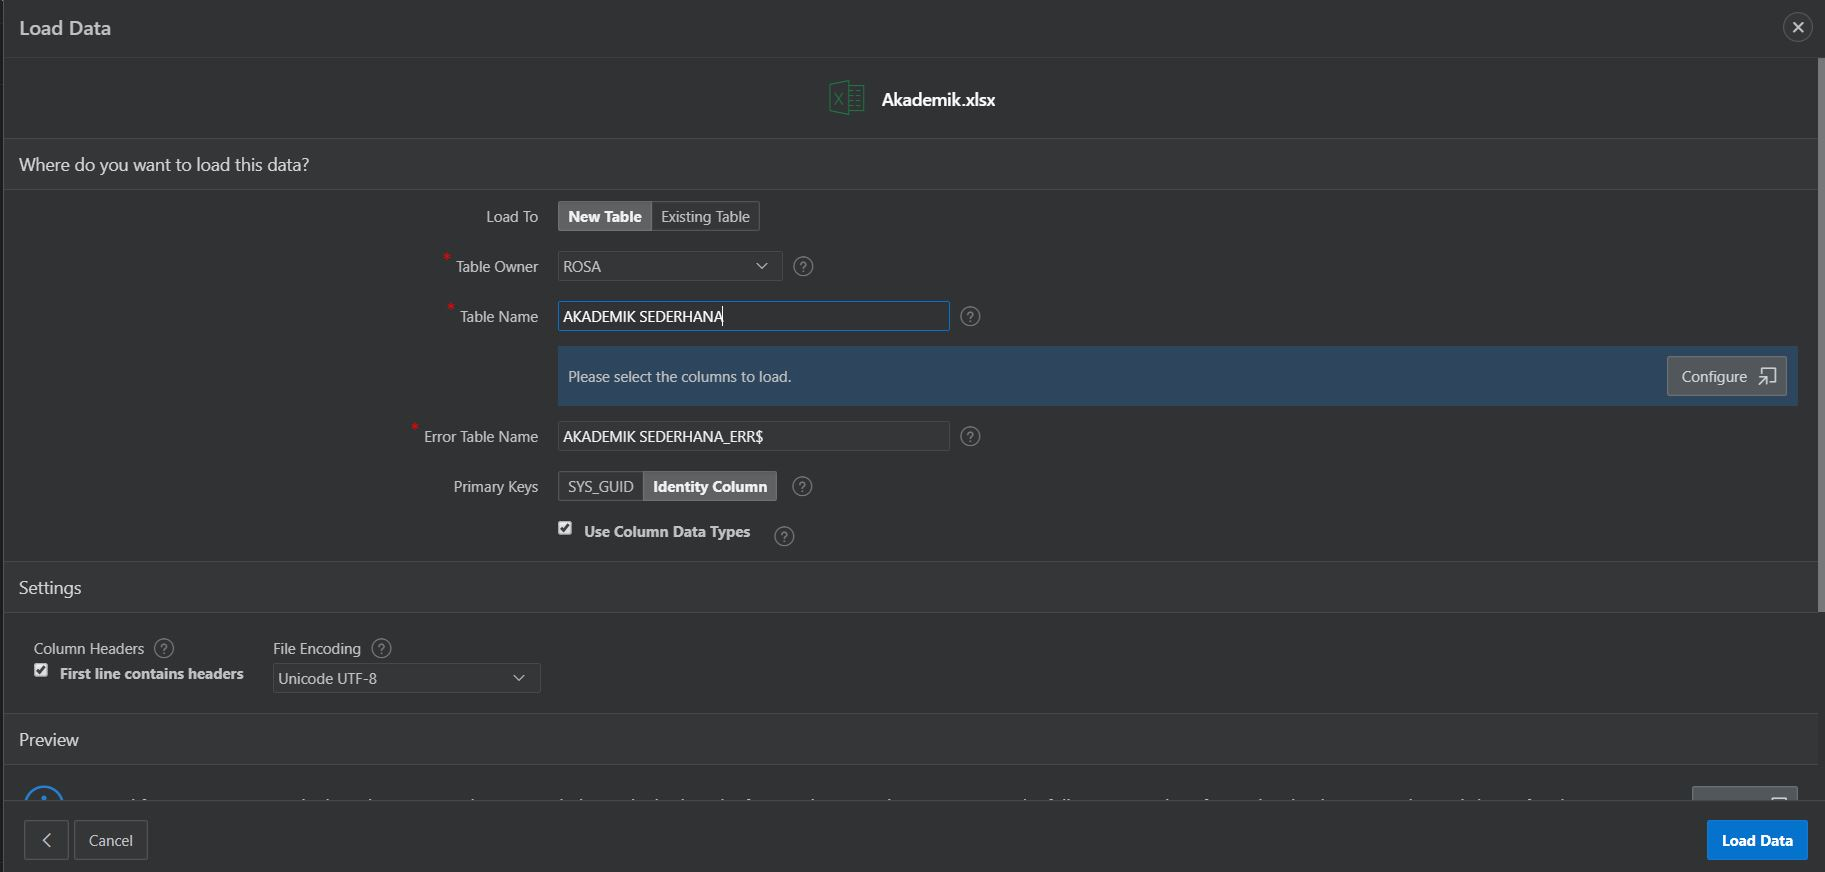
\includegraphics[scale=0.4]{section/7.JPG}
    \label{gambar 1}
\end{figure}

\item Setelah Sudah memuat data, tampilan selanjutnya akan seperti berikut.
       \begin{figure}[!htbp]
    \centering
    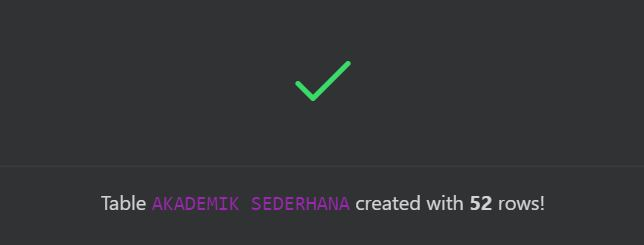
\includegraphics[scale=0.6]{section/9.JPG}
    \label{gambar 1}
\end{figure}

\item Load Data Sukses , klik Continue to Create Aplication.
\vspace{8cm}

\item Sekarang anda ada di tampilan Create an Aplication, ikuti langkah berikut, buat nama App from a Spreadsheet lalu pada Features klik Check All.
       \begin{figure}[!htbp]
    \centering
    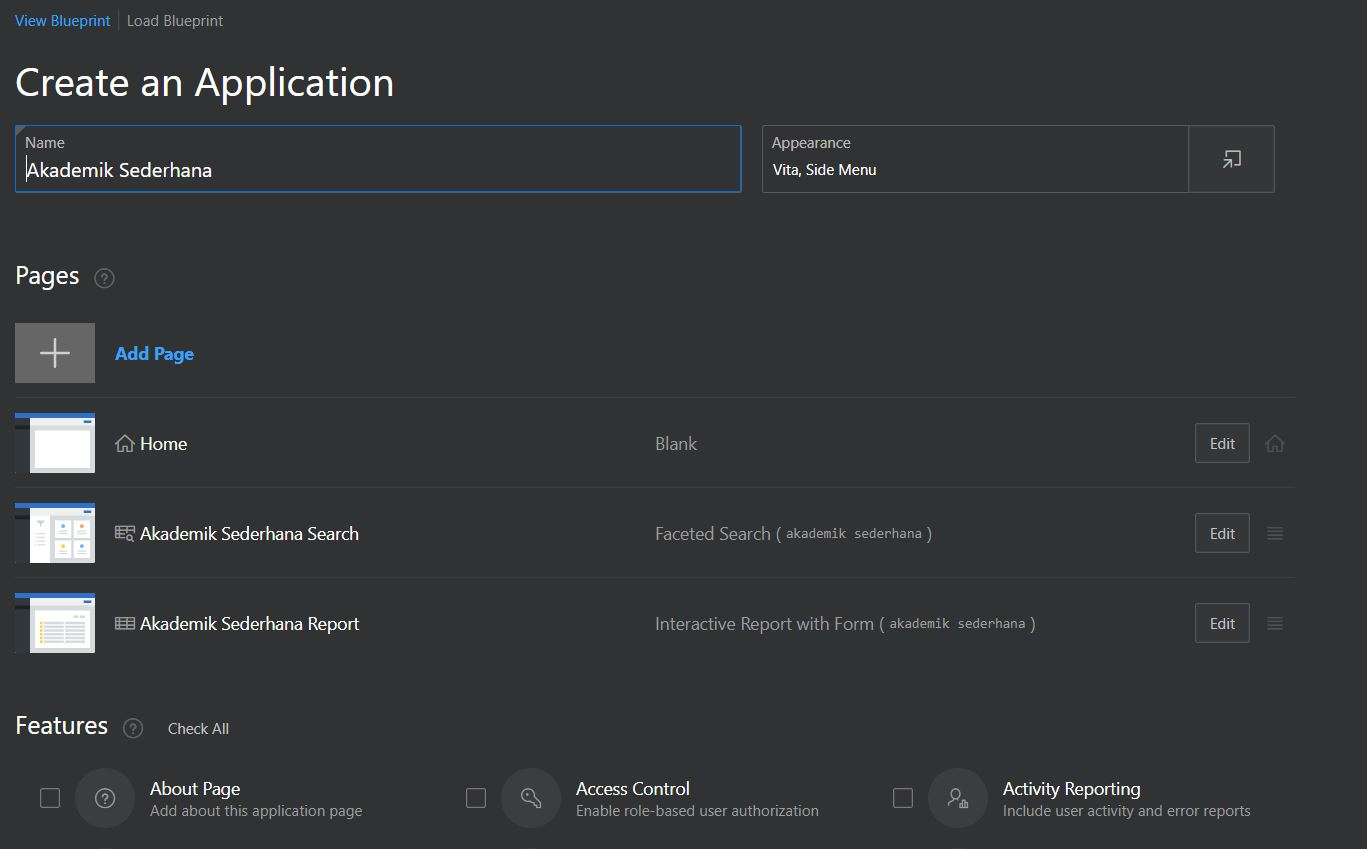
\includegraphics[scale=0.5]{section/10.JPG}
    \label{gambar 1}
\end{figure}


\item Scroll ke bawah lalu klik Create Application .
 

\item Tunggu sebentar, data sedang dimuat .
       \begin{figure}[!htbp]
    \centering
    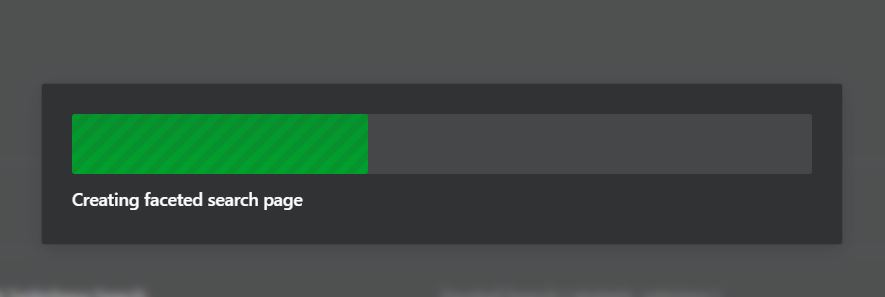
\includegraphics[scale=0.5]{section/11.JPG}
    \label{gambar 1}
\end{figure}

\item Anda akan masuk ke halaman App Builder project Spreadsheet telah berhasil dibuat !, lalu klik Run application .

\item Login ke Aplikasi anda menggunakan login Oracle APEX .

\item Selamat Aplikasi anda telah berjalan ! 
\item Link https://apex.oracle.com/pls/apex/f?p=79117:3:5595826331167::NO:::
\item WORKSPACE   : ROSA
\item EMAIL       : anisarosalina026@gmail.com
\item PASSWORD    : anisa1184016



  \begin{enumerate}
   
      
  \end{enumerate}
  \end{enumerate}
